\chapter{Introduction}

Stroke is the leading cause of disability, and neurorehabilitation aims to enhance brain plasticity to promote rapid recovery and restore lost motor functions. Functional Electrical Stimulation (FES) has been shown to improve rehabilitation outcomes. FES effectiveness increases when combined with a patient's voluntary effort, which current open-loop-based or triggered controllers fail to encourage in hospital or rehabilitation center settings.

Newer technologies are emerging, which use electromyography (EMG) sensors to capture muscle signals and encourage active patient contribution. Unfortunately, most of these devices are threshold-based or focus only on detecting the intention of movement, and lack the design of a controller with the ability to learn, generalize, and adapt not only to different stroke survivors but also to individual stroke survivors over time. Furthermore, while many studies have examined the importance of wrist flexion, not enough attention has been paid to arm flexion and the recovery of reaching movements.

In this context, the following crucial questions surface. These questions, while not directly addressed within the confines of the thesis, are essential to contextualize the significance and potential applications of this research. 

\begin{itemize}
    \item Is it possible to develop a technology that can provide FES stimulation tailored to each patient's current muscular activity?
    \item Is it feasible to create a system that can autonomously respond and adapt to a patient's input without any human interaction?
    \item Is it possible to create a framework that resembles the arm dynamics that will allow different control methods that comply with the previous questions to be tested?
\end{itemize}

In the attempt to start developing solutions to answer these questions this thesis presents a simulation framework to facilitate the evaluation of various controls that determine the arm's functional electrical stimulation input based on EMG signals. A proportional controller was used to test the framework's effectiveness, showing the potential and adaptability of this strategy. 

\section{Research Goals} \label{sec:reserachgoal}

This project aims to achieve the following goals. A flow diagram (Figure \ref{fig:researchgoals}) is presented below the research goals to show the connection between the different research goals and the three main objectives.

\begin{enumerate}

    \item \textbf{Identify Gaps in Current FES Technology}:
    \begin{itemize}
        \item Conduct an exhaustive literature review to recognize limitations and shortcomings in the present Functional Electrical Stimulation (FES) technology.
        \item Provide recommendations or potential avenues for advancement based on identified gaps.
    \end{itemize}
    
      \item \textbf{Analyze Current FES Control Methods}:
    \begin{itemize}
        \item Review and evaluate prevalent FES control methods and strategies from recent literature.
        \item Determine and select the most suitable control method for integration with this project based on performance, reliability, and compatibility metrics.
    \end{itemize}
    
    \item \textbf{Comprehend and Replicate an Established Model}:
    \begin{itemize}
        \item Understand the intricacies and functionalities of the chosen controller.
        \item Successfully replicate the dynamic arm simulator's movement using the aforementioned controller.
    \end{itemize}

    \item \textbf{Develop and Validate Arm Dynamics Model and Neural Modelling}:
    \begin{itemize}
        \item Design a model that will represent the arm dynamics.
        \item Record neural activity data from arm movement.
    \end{itemize}
    
    \item \textbf{Simulate Arm Movements Using Inverted Models}:
    \begin{itemize}
        \item Utilize the inverse of the models to simulate the arm's movement in the dynamic arm simulator.
        \item Test with different paths and movements.
    \end{itemize}
    
    \item \textbf{Integration of Neural activity Data}:
    \begin{itemize}
        \item Record artificially created neural activity data for varied arm movements.
        \item Incorporate this data into the simulator to enhance the authenticity and responsiveness of the arm's movements.
        \item Record arm movements simulated impaired neural activity, simulating stroke survivors movement.
    \end{itemize}
    
    \item \textbf{Develop an Additional Layer for an EMG-inspired Control}:
    \begin{itemize}
        \item Design and implement an additional layer in the control system to provide supplementary neural activity, resembling the FES devices, ensuring smooth and accurate arm movement that will resemble an impaired arm.
    \end{itemize}
\end{enumerate}


\begin{figure}[h!]
    \centering
    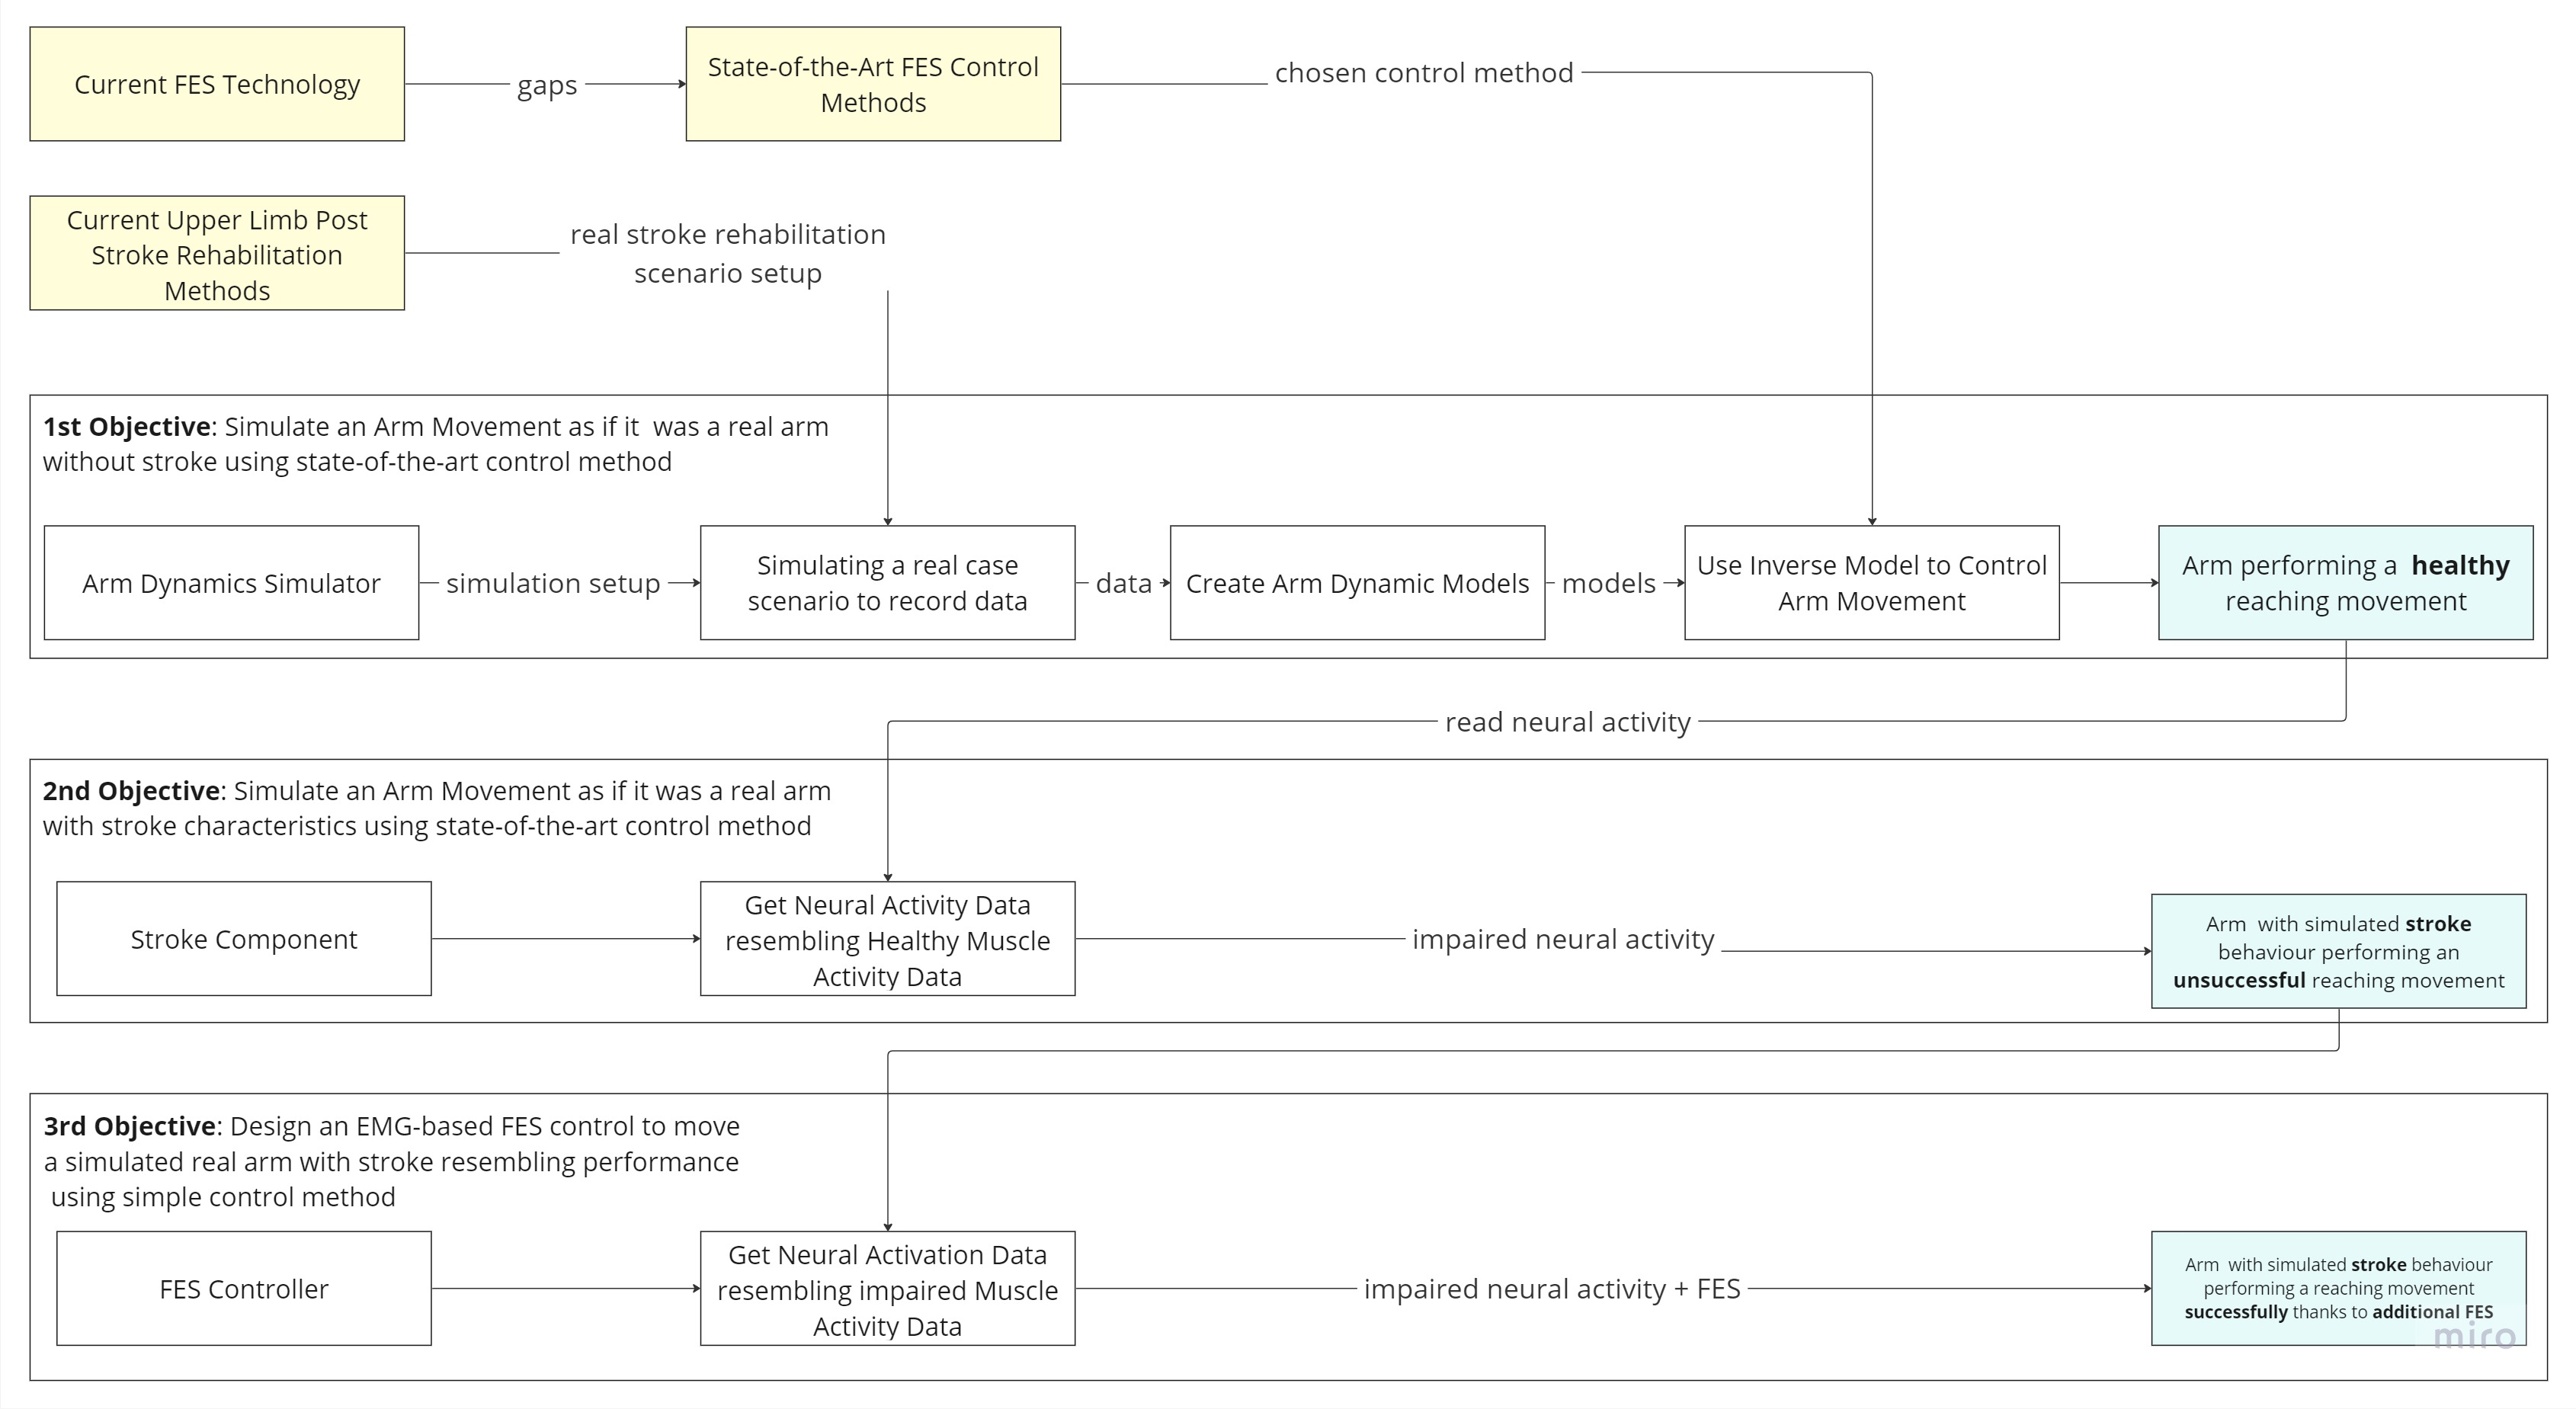
\includegraphics[width=\textwidth]{Pictures/ResearchGoals.jpg}
    \caption{Research Goals Flow Diagram }
    \label{fig:researchgoals}
\end{figure}


\section{Project Overview}

This thesis covers the process from understanding the research motivation to the detailed design, tool use, and model development needed to meet our goals.

It is structured in the following way:

\textbf{Chapter 1: Introduction} offers and initial dive into the central research question, the current existing gaps and the problem statement. Moreover it introduces the research goals that will be aimed to be completed along the thesis.

\textbf{Chapter 2: Motivation} serves as a backbone and clarifies the context of the research. The chapter shed light on contemporary FES technologies and their inherent drawbacks, starting with a general overview of the background and moving on to a detailed examination of post-stroke upper limb rehabilitation.

\textbf{Chapter 3: Design} The outline for the research is provided in this chapter. It states the design criteria, presents an initial design block diagram and the corresponding requirements for the experiment setup. It also presents in detail the tool employed in this study- a comprehensive model for musculoskeletal dynamics of the arm. 

\textbf{Chapter 4: Model Design and Development} dives in the intricacies of the arm dynamics model development. From defining the data used for the model to the creation of the Semi-Parametric Gaussian Process Regression model.

\textbf{Chapter 5: Control Design and Development} offers an in-depth analysis of different studies where multiple controllers were used for FES. A Quasi-Static Controller is chosen as the most fitted one or this project. In this chapter the controller is developed starting from a static position, then moving into a path-following quasi-static controller and finally into the novelty of adding the EMG-influenced controller.

\textbf{Chapter 6: Results} presents the findings from the Semi-Parametric GPR Models and the implemented stages of the controller.

\textbf{Chapter 8: Discussion and Future Work} critically evaluates the results, highlighting their implications and significance. A small sections of failed attempts is presented. Finally it paves the way forward, suggesting further directions this research can take.

\textbf{Chapter 9: Conclusion} wraps up the research, summarizing its key findings and their importance in the grand scheme of upper-limb stroke rehabilitation. 